\section{Experiments}

In this section, we conduct comprehensive experiments and report the experimental setup, main results, and ablation analyses. 
We answer the following research questions (RQs):
\textbf{RQ1:} Does GraphWalker outperform other LLM-based KGQA methods?
\textbf{RQ2:} Does GraphSynth broaden GraphWalker's search space and improve generalization?
\textbf{RQ3:} How does each training stage contribute to GraphWalker's final performance?
\textbf{RQ4:} How do the main components of our data construction pipeline work?


% ###################################################

\subsection{Experimental Setup}

\textbf{Datasets and Metrics.}
Following previous research \citep{sun2023think,luo2023reasoning}, we evaluate GraphWalker on two widely used KGQA benchmarks: CWQ \citep{talmor2018webknowledgebaseansweringcomplex} and WebQSP \citep{Yih2016TheVO}. To ensure a fair comparison, we utilize the gold topic entities provided by the benchmarks and report standard Exact Match (EM) and $F1$ scores \citep{talmor2018webknowledgebaseansweringcomplex}. Details of the datasets are described in Appendix~\ref{app:datasets}.



\textbf{Models and Baselines.}
We compare GraphWalker with seven previous prompting-based and training-based KGQA methods. 
% To ensure a fair comparison and reproducibility, we report the scores for these methods directly from their original publications.
To better evaluate the effectiveness of various methods on knowledge reasoning tasks, we use the full Freebase as a KG backend (\textit{Global KG} setting).
This setting is more challenging than approaches based on predefined subgraphs, as the agent must navigate the full KG.
For KG-R1, we evaluate the released checkpoint in the official repository under our Global KG setting. 
We additionally evaluate strong proprietary LLMs, including \texttt{DeepSeek-V3.2} and \texttt{GPT-4o-mini}, under the GraphWalker agent framework.
Details for all baselines are provided in Appendix~\ref{app:baselines}. 


\textbf{Implementation Details.}
We train and evaluate GraphWalker on three open-source backbone models: \textbf{Qwen2.5-3B-Instruct, Qwen2.5-7B-Instruct} \citep{qwen2025qwen25technicalreport}, and \textbf{Llama-3.1-8B-Instruct} \citep{dubey2024llama}.  
For SFT data collection, we use \texttt{GPT-4o-mini} to generate trajectories for both GraphSynth and GraphRoll. For evaluation, we set the max turn number $T = 10$.
Our training implementation details are shown in Appendix~\ref{app:training_details}.

% ###################################################

\subsection{Main Results (RQ1)}

\begin{table*}[t]
  \centering
  \scriptsize
  \caption{Performance comparison (in percentage) of KGQA methods on CWQ and WebQSP. The best and second-best results are shown in \textbf{bold} and \underline{underlined}, respectively.~ ${}^{\dagger}$ denotes models evaluated under the GraphWalker interaction framework with full global KG.}
  \vspace{-6pt}
  \label{tab:main-results}
  \setlength{\tabcolsep}{10pt}
  \renewcommand{\arraystretch}{1.1}
  \begin{tabular}{l|l|cc|cc}
  \toprule
  \multirow{2}{*}{\textbf{Method}}
  & \multirow{2}{*}{\textbf{Backbone}}
  & \multicolumn{2}{c|}{\textbf{CWQ}}
  & \multicolumn{2}{c}{\textbf{WebQSP}} \\
  & & \textbf{EM} & \textbf{F1} & \textbf{EM} & \textbf{F1} \\
  \midrule
  \rowcolor{gray!15}
  \multicolumn{6}{c}{\textit{Vanilla LLMs}} \\
  \midrule
  IO Prompt & Qwen2.5-3B-Instruct & 22.0 & 17.7 & 44.6 & 30.3 \\
  IO Prompt & Qwen2.5-7B-Instruct & 25.7 & 20.7 & 50.9 & 33.2 \\
  IO Prompt & GPT-4o-mini & 45.5 & 33.6 & 47.1 & 39.3 \\
  IO Prompt & DeepSeek-V3.2 & 50.1 & 43.5 & 63.8 & 55.7 \\
  \midrule
  \rowcolor{gray!15}
  \multicolumn{6}{c}{\textit{Agentic KGQA Methods}} \\
  \midrule
  RoG & LLaMA-2-7B-Instruct & 62.6 & 56.2 & 85.7 & 70.8 \\
  ToG & GPT-4 & 69.5 & - & 81.9 & - \\
  ToG-2.0 & GPT-3.5 & 68.9 & 65.8 & 77.8 & 74.5 \\
  GoG & GPT-4 & 75.2 & - & 84.4 & - \\
  KBQA-o1 & LLaMA3.1-8B-Instruct& - & - & 75.8 & 82.1 \\
  KG-Agent & LLaMA2-7B-Instruct & 72.2 & \underline{69.8} & 83.3 & 81.0 \\
  ${}^{\dagger}$KG-R1 & Qwen2.5-3B-Instruct & 66.8 & 61.7 & 82.1 & 78.9 \\
  \midrule
  \rowcolor{gray!15}
  \multicolumn{6}{c}{\textit{GraphWalker (Our Method)}} \\
  \midrule
  ${}^{\dagger}$Vanilla Agent
    & Qwen2.5-7B-Instruct
    & 40.7 & 33.2
    & 68.4 & 66.1 \\
  ${}^{\dagger}$Vanilla Agent
    & GPT-4o-mini
    & 63.4 & 60.3
    & 79.6 & 70.6 \\
  ${}^{\dagger}$Vanilla Agent
    & DeepSeek-V3.2
    & 69.8 & 63.5
    & 76.7 & 71.8 \\
  \rowcolor{blue!8}
  GraphWalker-7B-SFT
    & Qwen2.5-7B-Instruct
    & 68.3 & 63.2 & 82.0 & 79.1 \\
  \rowcolor{blue!8}
  GraphWalker-3B-SFT-RL
    & Qwen2.5-3B-Instruct
    & 70.9 & 65.2 & 83.5 & 81.7 \\
  \rowcolor{blue!8}
  GraphWalker-8B-SFT-RL
    & LLaMA3.1-8B-Instruct
    & \underline{78.5} & 69.6 & \underline{88.2} & \underline{84.5} \\
  \rowcolor{blue!15}
  \textbf{GraphWalker-7B-SFT-RL}
    & Qwen2.5-7B-Instruct
    & \textbf{79.6} & \textbf{74.2}
    & \textbf{91.5} & \textbf{88.6} \\
  \bottomrule
  \end{tabular}
  \vspace{-16pt}
\end{table*}


As shown in Table~\ref{tab:main-results}, GraphWalker achieves SOTA performance across all benchmarks, demonstrating its effectiveness from two perspectives:

\textbf{Superiority in Complex Reasoning.} 
GraphWalker consistently outperforms both prompting and training baselines.
Notably, it surpasses the GPT-4-powered GoG by 4.4\% EM on CWQ, and outperforms training-based models such as KG-Agent (+7.4\% EM on CWQ) and KBQA-o1 (+15.7\% EM on WebQSP).
Under the more challenging Global KG setting, GraphWalker-3B-SFT-RL outperforms KG-R1 (same \texttt{Qwen2.5-3B-Instruct} backbone) by a clear margin (e.g., +4.1\% EM on CWQ), suggesting that KG-R1's reliance on pre-extracted subgraphs undermines its robustness.
Moreover, equipping proprietary LLMs (\texttt{GPT-4o-mini} and \texttt{DeepSeek-V3.2}) with our interaction framework yields substantial gains over their IO Prompt counterparts (+17.9\% and +19.7\% EM on CWQ). 
Impressively, GraphWalker with trained backbones outperforms these proprietary LLMs across all model sizes, demonstrating the effectiveness of our synthetic agentic curriculum and training strategy.


\textbf{Cross-task Transferability.} Despite being trained solely on CWQ, GraphWalker effectively zero-shot transfers to WebQSP (91.5\% EM), outperforming all baselines trained directly on WebQSP data. This confirms that training on CWQ's structurally diverse, high-complexity paths equips the agent with highly transferable exploration strategies.






% ###################################################
\subsection{Comparison Analysis (RQ2)}

\begin{wrapfigure}{r}{0.36\linewidth}
    \centering
    \vspace{-4.8em}
    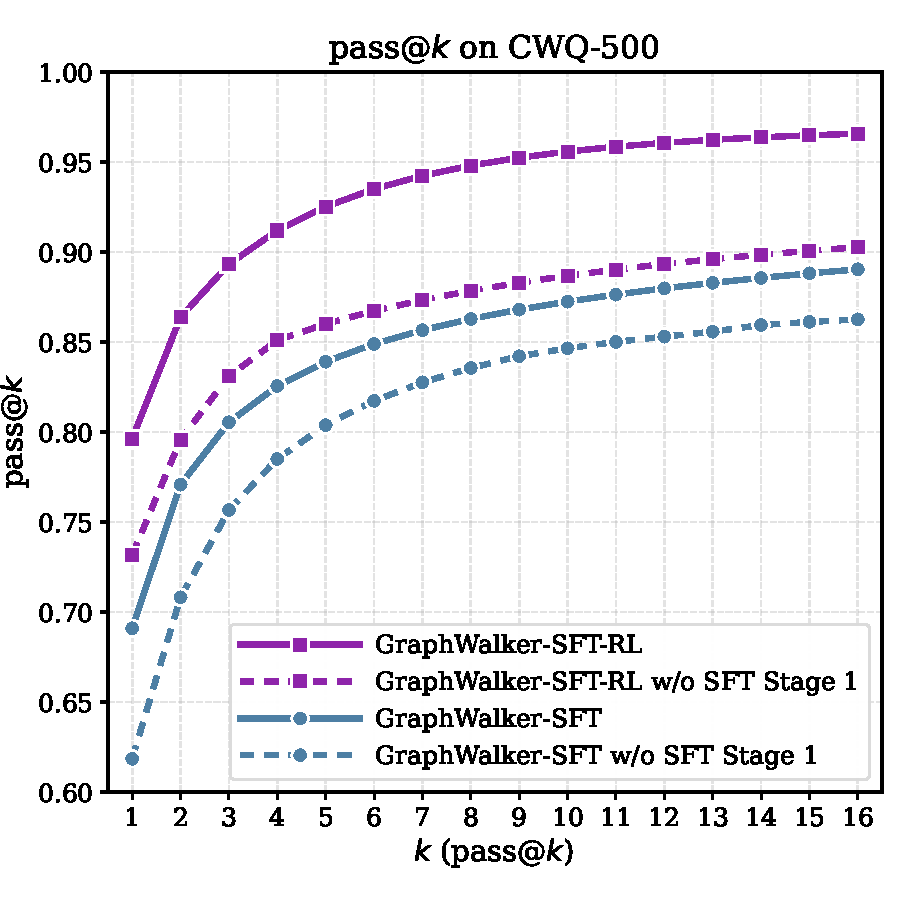
\includegraphics[width=\linewidth]{figures/pass_at_k_curve.pdf}
    \vspace{-2.2em}
    \caption{Pass@$k$ comparison.}
    \label{fig:passk}
    \vspace{-2.0em}
\end{wrapfigure}

\textbf{Pass@$k$ Analysis.}
To validate that GraphSynth effectively broadens the agent's reasoning search space, we sample 500 questions from the CWQ test set and evaluate exploration capacity via \textbf{Pass@$k$} over $32$ runs.
As shown in Figure~\ref{fig:passk}, within both the SFT-only and SFT-RL settings, removing GraphSynth (\textbf{w/o SFT Stage 1}) consistently reduces Pass@$k$ across all $k$, confirming its critical role in expanding the agent's exploration capacity. In contrast, models trained with GraphSynth exhibit higher Pass@$k$ values as $k$ increases, indicating that our CRW synthesis establishes a broader exploration prior. 
Furthermore, \textbf{GraphWalker-SFT-RL} achieves the highest Pass@$k$ across all $k$, suggesting that a stronger exploration foundation enables RL to further amplify these gains.


\textbf{Zero-shot Generalization.}
To assess whether GraphSynth improves reasoning generalization, we evaluate GraphWalker and its ablated variants on two zero-shot benchmarks: the zero-shot split of \textit{GrailQA} and \textit{GraphWalkerBench}, a structurally diverse evaluation set involving unseen reasoning structures not present in GraphSynth (see Appendix~\ref{app:datasets}).
As shown in Table~\ref{tab:zeroshot}, both SFT stages are crucial for out-of-distribution (OOD) generalization. Removing GraphSynth (\textbf{w/o SFT Stage 1}) significantly impairs generalization (6.80\% average EM drop), confirming its essential role in broadening the agent's search space. 
Similarly, removing GraphRoll (\textbf{w/o SFT Stage 2}) leads to substantial performance degradation (11.10\% average EM drop), as the model's ability to self-correct is significantly weakened. Furthermore, the consistent improvement of \textit{GraphWalker-Full} over \textit{w/o RL} confirms that RL further enhances the generalization capability established by the SFT stages.



\begin{table}[t]
\centering
\scriptsize
\setlength{\tabcolsep}{3pt}
\renewcommand{\arraystretch}{1.1}
\begin{minipage}[t]{0.44\linewidth}
\centering
\caption{Zero-shot performance on \textit{Grail-}\\\textit{QA} and \textit{GraphWalkerBench}, which involves unseen structures in \textit{GraphSynth}.}
\label{tab:zeroshot}
\begin{tabular}{cccccc}
\toprule
\multirow{2}{*}{Method} & \multicolumn{2}{c}{GrailQA} 
& \multicolumn{2}{c}{\makecell{GraphWalker\\Bench}}
& \multirow{2}{*}{$\Delta~\overline{\text{EM}}$} \\
\cmidrule(lr){2-3} \cmidrule(lr){4-5}
& EM & F1 & EM & F1 & \\
\midrule
\rowcolor{blue!8}
\textbf{GraphWalker-Full} & \textbf{86.3} & \textbf{84.4} & \textbf{63.5} & \textbf{60.8} & --- \\
\midrule
\rowcolor{gray!15}
\multicolumn{6}{c}{\textit{Ablations}} \\
\midrule
w/o SFT Stage 1 & 80.9 & 78.0 & 55.3 & 52.4 & $-$6.80 \\
w/o SFT Stage 2 & 74.3 & 69.7 & 53.3 & 49.5 & $-$11.10 \\
w/o RL          & 79.4 & 76.3 & 49.7 & 47.0 & $-$10.35 \\
\bottomrule
\end{tabular}
\end{minipage}
\hfill
\begin{minipage}[t]{0.54\linewidth}
\centering
\caption{Ablation study on \textit{CWQ} and \textit{WebQSP}.}
\label{tab:phase_ablation}
\vspace{-8pt}
\begin{tabular}{ccccccc}
\toprule
\multirow{2}{*}{Method} & \multicolumn{2}{c}{CWQ} & \multicolumn{2}{c}{WebQSP}
& \multirow{2}{*}{$\Delta~\overline{\text{EM}}$} \\
\cmidrule(lr){2-3} \cmidrule(lr){4-5}
& EM & F1 & EM & F1 & \\
\midrule
\rowcolor{blue!8}
\textbf{GraphWalker-Full}
& \textbf{79.6} & \textbf{74.2}
& \textbf{91.5} & \textbf{88.6} & --- \\
\midrule
\rowcolor{gray!15}
\multicolumn{6}{c}{\textit{Training Stage Ablations}} \\
\midrule
w/o SFT Stage 1 & 75.2 & 70.4 & 85.7 & 82.5 & $-$5.10 \\
w/o SFT Stage 2 & 72.3 & 66.3 & 80.8 & 77.5 & $-$9.00 \\
w/o SFT         & 70.6 & 66.0 & 79.8 & 75.6 & $-$10.35 \\
w/o RL          & 68.3 & 63.2 & 82.0 & 79.1 & $-$10.40 \\
\midrule
\rowcolor{gray!15}
\multicolumn{6}{c}{\textit{Training Order Ablation}} \\
\midrule
Mixed-SFT+RL  & 70.2 & 64.2 & 80.1 & 75.8 & $-$10.40 \\
\bottomrule
\end{tabular}
\end{minipage}
\vspace{-10pt}
\end{table}



% ###################################################


\subsection{Analysis on Each Training Stage (RQ3)}



\textbf{Ablation of Each Stage.}
To understand the contribution of each training stage, we ablate 
individual components from the training pipeline.
As shown in Table~\ref{tab:phase_ablation}, removing GraphSynth (\textbf{w/o SFT Stage 1}) causes a substantial decline (5.10\% average EM drop), indicating its critical role in establishing broad exploration priors for navigating complex KG structures. 
Meanwhile, removing GraphRoll (\textbf{w/o SFT Stage 2}) leads to an even greater drop (9.00\% average EM drop), demonstrating that 
GraphRoll's expert trajectories are essential for instilling reflection and self-correction capabilities. 
Finally, removing RL results in a severe 10.40\% average 
EM drop, confirming that RL further consolidates the capabilities 
established by the SFT stages.



\textbf{Importance of Stage-wise Training.}
To validate the proposed curriculum, we compare stage-wise training against a \textbf{Mixed} baseline combining GraphSynth and GraphRoll into a single SFT pass with identical RL training. As shown in Table~\ref{tab:phase_ablation}, mixed training consistently underperforms (dropping from 79.6\% to 70.2\% EM on CWQ) despite using identical data, confirming that training order is critical: 
Stage 1 must first establish broad exploration priors before Stage 2 
can effectively instill reflection and recovery capabilities.


% ##############################################################





\subsection{Ablation Study (RQ4)}

To better understand the internal mechanisms of GraphWalker, we conduct ablation experiments on key components of our pipeline.


\begin{wrapfigure}{r}{0.48\linewidth}
    \centering
    \vspace{-3.2em}
    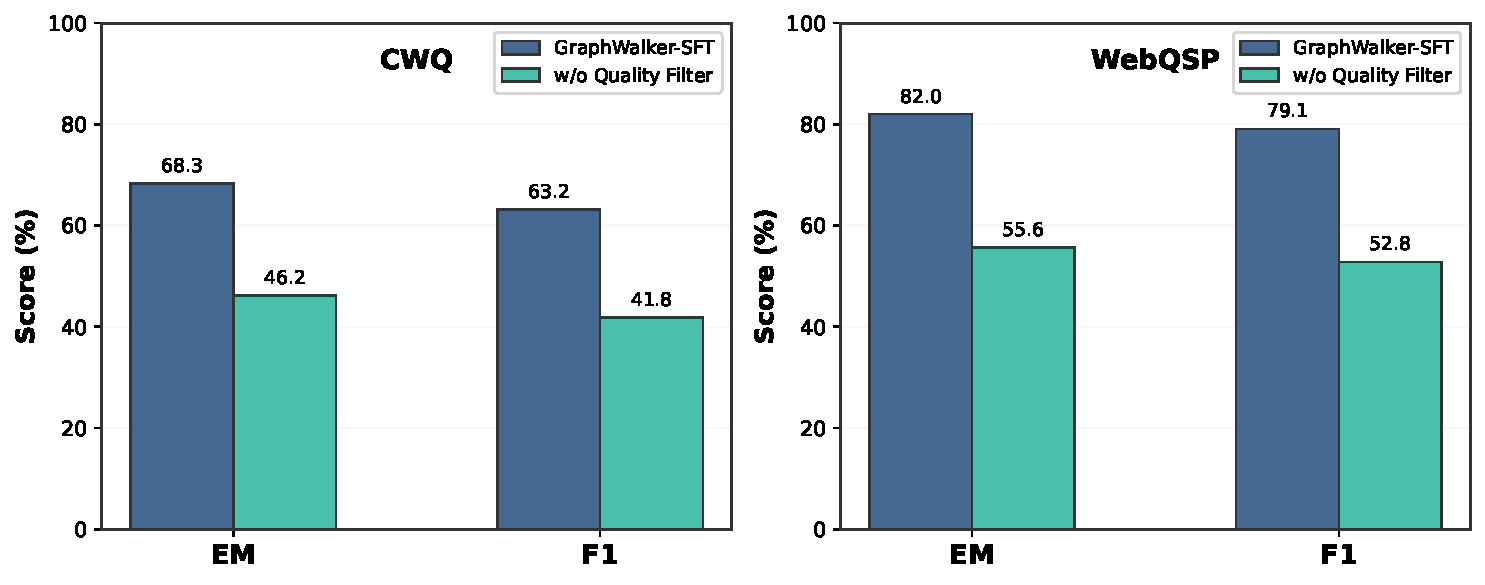
\includegraphics[width=\linewidth]{figures/ablation_comparison.pdf}
    \vspace{-2.2em}
    \caption{Ablation study on the \textit{quality filter}.}
    \label{fig:ablation}
    \vspace{-2.4em}
\end{wrapfigure}

\textbf{Impact of Quality Filtering.}
As shown in Figure~\ref{fig:ablation}, removing the \textit{quality filter} from the GraphWalker-SFT model causes substantial performance drops on both datasets: EM drops from 68.3\% to 46.2\% on CWQ and from 82.0\% to 55.6\% on WebQSP, confirming that filtering out low-quality questions is critical to the overall data pipeline.




% ###################################################


\textbf{Impact of Data Scale.}

\begin{figure}[t]
    \centering
    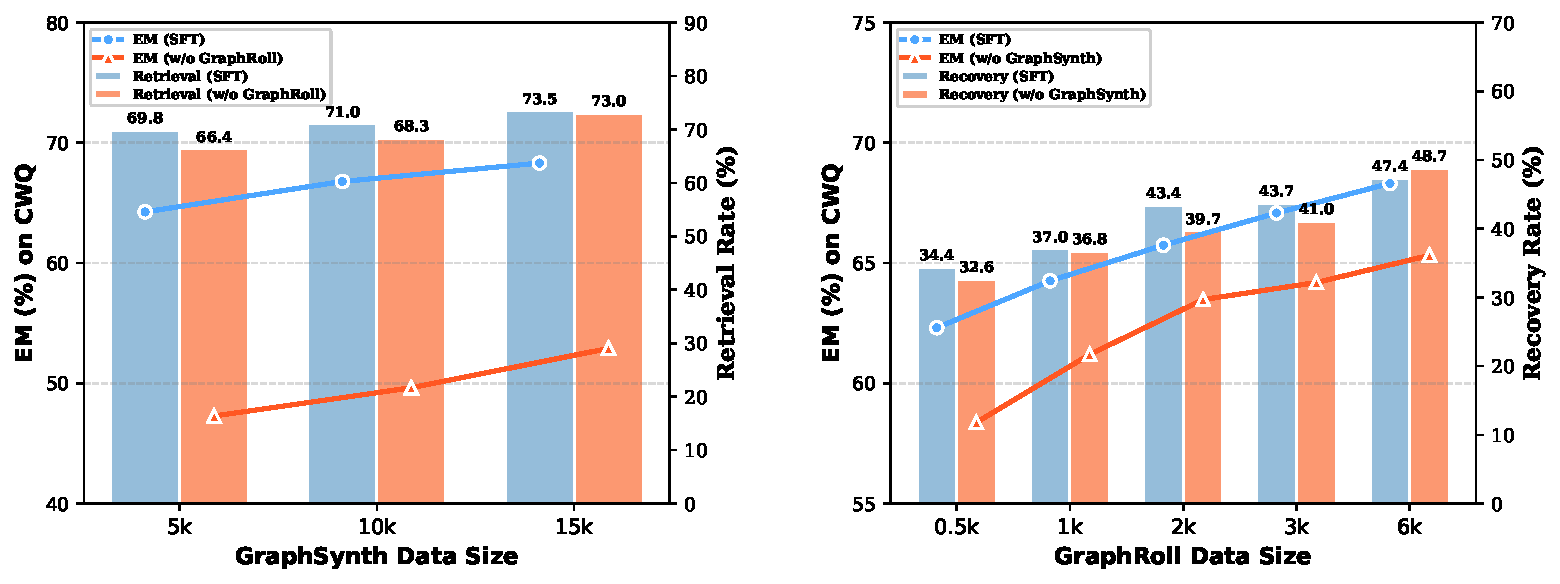
\includegraphics[width=0.90\linewidth]{figures/scaling_plot.pdf}
    \caption{
    Impact of data scale on performance.
    \textit{Left}: scaling GraphSynth data improves \textit{EM} and \textit{Retrieval Rate}.
    \textit{Right}: scaling GraphRoll data improves \textit{EM} and \textit{Recovery Rate}.
    }
    \label{fig:scaling}
    \vspace{-18pt}
\end{figure}

We investigate the effect of data scale on each training stage separately.
For Stage 1, we vary the size of GraphSynth across $\{5\text{k}, 10\text{k}, 15\text{k}\}$ samples; for Stage 2, we vary GraphRoll across $\{0.5\text{k}, 1\text{k}, 2\text{k}, 3\text{k}, 6\text{k}\}$ samples. 
Here, \textit{Retrieval Rate} measures the proportion of test cases where the gold answer appears in the agent's retrieved observations, reflecting the agent's ability to find relevant evidence through KG exploration; 
\textit{Recovery Rate} measures the proportion of cases where the 
agent successfully corrects an erroneous \texttt{<kg-query>} step 
and recovers to the correct answer.
As shown in Figure~\ref{fig:scaling}, both \textit{EM} and the corresponding \textit{Retrieval/Recovery Rates} improve consistently with data scale, confirming the benefit of scaling trajectory supervision. 
Notably, the performance gap between the full model and the ablated variants (\textbf{w/o GraphRoll} and \textbf{w/o GraphSynth}) persists across all scales, demonstrating that the two stages provide complementary and irreplaceable contributions.


% ###################################################



